\section{实验环境建立}
\subsection{VMWARE下中文UBUNTU安装(5分)}
安装Ubuntu,安装中文输入法(搜狗输入法),用户名为学号。

打开终端term,输入Hello 1160300202冯云龙。

截图:要求有Windows状态行,Vmware窗口,Ubuntu窗口,终端term窗口,输入的“Hello 1160300202冯云龙”信息。

\begin{figure}[H]
	\centering
	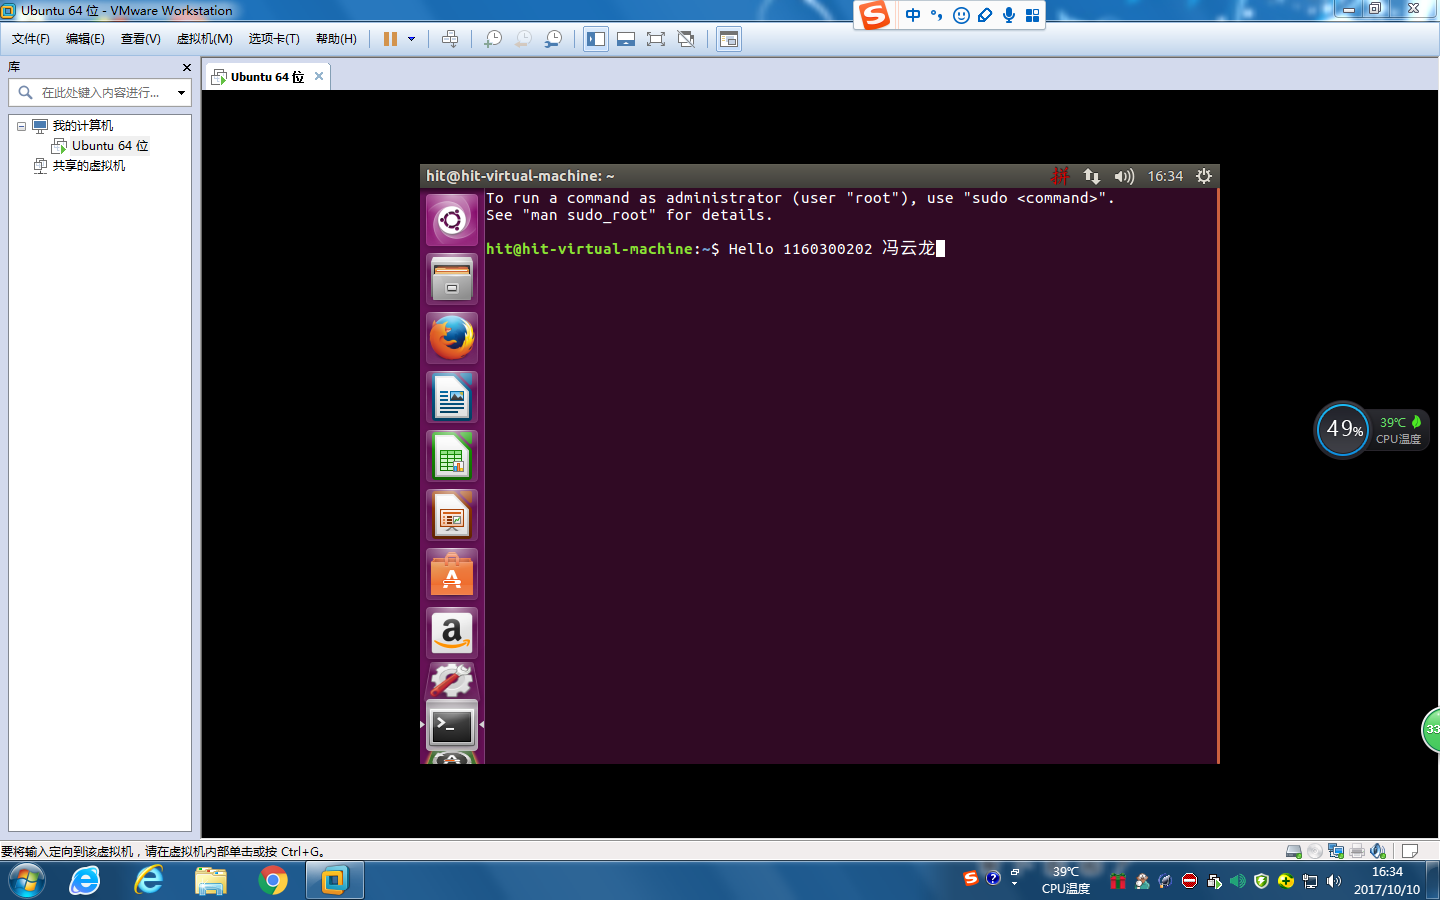
\includegraphics[width=0.55\linewidth]{figures/VM-Ubuntu}
	\caption{Vmware下中文Ubuntu安装效果截图}
	\label{fig:vm-ubuntu}
\end{figure}

\subsection{UBUNTU与WINDOWS目录共享(5分)} 

在Windows下建立一目录,将hellowin.c拷贝到此目录。在vmware下设置Ubuntu共享hitics。

在Ubuntu下Home建立快捷链接hitics指向此共享目录,并在此目录建立hellolinux.c。

打开终端term,进入此目录,输入 “ls –la” 指令。

截图:要求有Ubuntu的“文件”应用打开“Home”,能看到hitics。term窗口。


\begin{figure}[H]
	\centering
	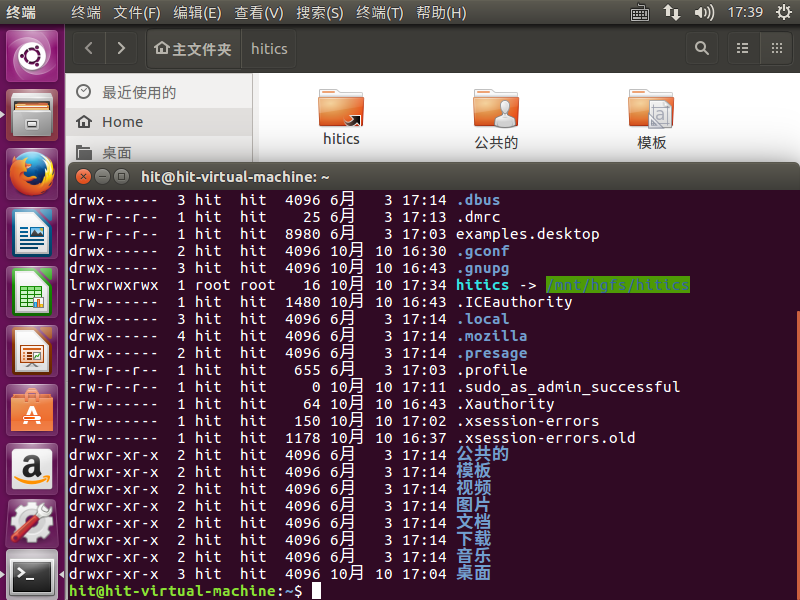
\includegraphics[width=0.5\linewidth]{figures/VM-Win-Lin-Share}
	\caption{Vmware下中文Ubuntu安装效果截图}
	\label{Ubuntu与Windows共享目录截图}
\end{figure}

